% bitsian_multivar_tut3_detailed.tex
% Tutorial Sheet 3 Solutions - Detailed BITS Style with Insight Boxes
% Compile with XeLaTeX (Required for fontspec)

\documentclass[11pt,a4paper]{article}
\usepackage[a4paper,margin=1in]{geometry}
\usepackage{microtype}
% navigation / bookmarks
\usepackage{bookmark}
\setcounter{tocdepth}{1} % Show sections in TOC

% Fonts - Matching your preferred aesthetic
\usepackage{fontspec}
\setmainfont{TeX Gyre Termes}
\newfontfamily\uiSans{Inter}[Scale=0.98]
\IfFontExistsTF{Kalam}{\newfontfamily\handfont{Kalam}[Scale=0.95]}{\newcommand{\handfont}{}}

% Math
\usepackage{amsmath,amssymb,mathtools}

% Graphics + float control
\usepackage{graphicx}
\usepackage{float}
\usepackage{placeins}
\usepackage{caption}
\captionsetup{font=small,labelfont=bf}

% Colors - The BITSian Palette
\usepackage{xcolor}
\definecolor{ink}{HTML}{1C1E21}
\definecolor{muted}{HTML}{6B7280}
\definecolor{accentA}{HTML}{8A5CF6}   % purple
\definecolor{accentB}{HTML}{FF7A59}   % orange
\definecolor{chip}{HTML}{00C2A8}      % teal chip
\definecolor{noteY}{HTML}{FFF2B2}     % sticky yellow
\definecolor{dot}{HTML}{D4D6DA}       % dot grid color (very light)

% Links
\usepackage{hyperref}
\hypersetup{colorlinks=true,linkcolor=muted,urlcolor=accentA,citecolor=muted}

% TikZ dotted background
\usepackage{tikz,eso-pic}
\usetikzlibrary{calc}
\newcommand{\dotstep}{6mm}
\newcommand{\dotradius}{0.35pt}
\newcommand{\dotopacity}{0.14}

\AddToShipoutPictureBG{%
  \begin{tikzpicture}[remember picture,overlay]
    \def\xstart{1in}
    \def\ystart{-1in}
    % Cover the whole page with dots
    \foreach \i in {0,...,35} {
      \foreach \j in {0,...,50} {
        \fill[black!70,opacity=\dotopacity]
          ($(current page.north west)+(\xstart + \i*\dotstep,\ystart - \j*\dotstep)$)
          circle (\dotradius);
      }
    }
  \end{tikzpicture}%
}

% Header / footer
\usepackage{fancyhdr}
\pagestyle{fancy}
\fancyhf{}
\lhead{\small\uiSans Math F111 — Tutorial 3}
\rhead{\small\uiSans Vector Calculus: Curves \& Motion}
\cfoot{\small\thepage}

% --- THE YELLOW STICKY NOTE ---
\usepackage{tcolorbox}
\tcbuselibrary{skins,breakable}
\tcbset{enhanced,frame hidden,sharp corners,colback=white,boxsep=6pt}

\newtcolorbox{StickyNote}[1][]{
  enhanced, breakable,
  colback=noteY,
  borderline west={2.5pt}{0pt}{accentB!90}, % Thicker orange line
  drop shadow={opacity=0.12,shadow xshift=1pt,shadow yshift=-1pt},
  title={\textbf{#1}}, % Optional title
  coltitle=ink,
  attach title to upper={\par\vspace{4pt}},
  fonttitle=\uiSans\small\bfseries,
  fontupper=\small\color{ink}
}

% Margin Step Marker
\usepackage{marginnote}
\reversemarginpar
\newcounter{step}
\newcommand{\Step}[1]{%
  \par\refstepcounter{step}%
  \marginnote{%
    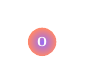
\begin{tikzpicture}
      \shade[inner color=accentA!90,outer color=accentB!90] (0,0) circle (0.18);
      \node[white,font=\bfseries\tiny] at (0,0) {\thestep};
    \end{tikzpicture}%
  }[-6pt]%
  \noindent\textbf{#1.}\,
}

% Problem header - Auto-TOC included
\newcommand{\Problem}[2]{%
  \phantomsection % create anchor for hyperref
  \addcontentsline{toc}{section}{Problem #1 — #2}% Add to TOC
  \vspace{18pt}%
  {\Large\uiSans\bfseries Problem #1}\hspace{0.6em}%
  {\setlength{\fboxsep}{3pt}\colorbox{chip!22}{\uiSans\footnotesize\textcolor{ink}{#2}}}\par
  \vspace{6pt}
  \setcounter{step}{0} % Reset steps for new problem
}

% Question Box Style
\newcommand{\QuestionText}[1]{%
    \vspace{4pt}
    \begin{tcolorbox}[colback=gray!5, colframe=gray!20, sharp corners, boxrule=0.5pt]
    {\small\itshape\color{ink!90} \textbf{Q:} #1}
    \end{tcolorbox}
    \vspace{4pt}
}

% Title
\title{\vspace{-6pt}\uiSans\bfseries Tutorial Sheet 3 — Solutions\\}
\author{}
\date{}

\begin{document}
\maketitle

% --- TOC ---
\tableofcontents
\clearpage
% -----------

{\color{muted}\rule{\linewidth}{0.6pt}}
\vspace{6pt}

% ======================================================================================
% PROBLEM 1
% ======================================================================================
\Problem{1}{Smoothness \& Vector Angles}
\QuestionText{Consider the space curve $r(t)=(1+\sin t)i+(t^{2}+\cos t)j+(t^{3}-\pi t^{2})k$, $t\ne0$ and $r(0)=0$. Find all points where $r(t)$ is smooth. Find the angle between the tangent and acceleration vectors at $t=\pi$.}

\Step{Condition for Smoothness}
A curve $\mathbf{r}(t)$ is smooth at a point if:
1. $\mathbf{r}'(t)$ exists and is continuous.
2. $\mathbf{r}'(t) \neq \mathbf{0}$. (The particle never stops moving).

\Step{Calculate Derivative $\mathbf{r}'(t)$}
\[ \mathbf{r}(t) = \langle 1+\sin t, t^2+\cos t, t^3-\pi t^2 \rangle \]
\[ \mathbf{v}(t) = \mathbf{r}'(t) = \langle \cos t, 2t - \sin t, 3t^2 - 2\pi t \rangle \]
This derivative exists for all $t \neq 0$.
Now, check if $\mathbf{r}'(t) = \mathbf{0}$. We need all three components to be zero simultaneously:
\begin{itemize}
    \item z-component: $t(3t - 2\pi) = 0 \implies t=0$ or $t=2\pi/3$.
    \item Check $t=2\pi/3$ in x-component: $\cos(2\pi/3) = -0.5 \neq 0$.
\end{itemize}
Since components are never zero at the same time for $t \neq 0$, the curve is smooth for all $t \neq 0$.
However, the problem states $\mathbf{r}(0)=\mathbf{0}$. As $t \to 0$, $\mathbf{r}(t) \to \langle 1, 1, 0 \rangle \neq \mathbf{0}$.
Since the function is discontinuous at $t=0$, it cannot be smooth there.
\textbf{Conclusion:} Smooth for all $t \in \mathbb{R} \setminus \{0\}$.

\Step{Angle at $t=\pi$}
Angle $\theta$ formula: $\cos \theta = \frac{\mathbf{v} \cdot \mathbf{a}}{|\mathbf{v}| |\mathbf{a}|}$.
Calculate vectors at $t=\pi$:
\begin{itemize}
    \item $\mathbf{v}(\pi) = \langle \cos \pi, 2\pi - \sin \pi, 3\pi^2 - 2\pi^2 \rangle = \langle -1, 2\pi, \pi^2 \rangle$.
    \item Acceleration $\mathbf{a}(t) = \mathbf{r}''(t) = \langle -\sin t, 2-\cos t, 6t - 2\pi \rangle$.
    \item $\mathbf{a}(\pi) = \langle 0, 2 - (-1), 6\pi - 2\pi \rangle = \langle 0, 3, 4\pi \rangle$.
\end{itemize}

\Step{Dot Product & Magnitudes}
\[ \mathbf{v} \cdot \mathbf{a} = (-1)(0) + (2\pi)(3) + (\pi^2)(4\pi) = 6\pi + 4\pi^3 \]
\[ |\mathbf{v}| = \sqrt{1 + 4\pi^2 + \pi^4} \quad \text{and} \quad |\mathbf{a}| = \sqrt{0 + 9 + 16\pi^2} \]
\[ \theta = \cos^{-1} \left( \frac{6\pi + 4\pi^3}{\sqrt{1+4\pi^2+\pi^4} \sqrt{9+16\pi^2}} \right) \]

\begin{StickyNote}[Exam Tip: Smoothness]
Students often check the derivative but forget to check if the derivative becomes the \textbf{zero vector}. A curve with a sharp corner (cusp) has $\mathbf{r}'(t) = \mathbf{0}$ at the cusp.
\end{StickyNote}

% ======================================================================================
% PROBLEM 2
% ======================================================================================
\Problem{2}{Initial Value Problem (IVP)}
\QuestionText{Solve the IVP: $\frac{d^{2}r}{dt^{2}}=-(i+j+k)$, $r(0)=ai+bj+ck$, $\frac{dr}{dt}|_{t=0}=0$.}

\Step{Integrate Acceleration ($\mathbf{a} \to \mathbf{v}$)}
$\mathbf{a}(t) = \langle -1, -1, -1 \rangle$.
Integrate with respect to $t$:
\[ \mathbf{v}(t) = \int \mathbf{a}(t) dt = \langle -t, -t, -t \rangle + \mathbf{C}_1 \]
Use Initial Condition: $\mathbf{v}(0) = \mathbf{0}$.
\[ \langle 0,0,0 \rangle + \mathbf{C}_1 = \mathbf{0} \implies \mathbf{C}_1 = \mathbf{0}. \]
So, $\mathbf{v}(t) = \langle -t, -t, -t \rangle$.

\Step{Integrate Velocity ($\mathbf{v} \to \mathbf{r}$)}
\[ \mathbf{r}(t) = \int \mathbf{v}(t) dt = \langle -\frac{t^2}{2}, -\frac{t^2}{2}, -\frac{t^2}{2} \rangle + \mathbf{C}_2 \]
Use Initial Condition: $\mathbf{r}(0) = \langle a, b, c \rangle$.
\[ \langle 0,0,0 \rangle + \mathbf{C}_2 = \langle a, b, c \rangle \implies \mathbf{C}_2 = \langle a, b, c \rangle. \]

\Step{Final Solution}
\[ \boxed{\mathbf{r}(t) = \left( a - \frac{t^2}{2} \right)\mathbf{i} + \left( b - \frac{t^2}{2} \right)\mathbf{j} + \left( c - \frac{t^2}{2} \right)\mathbf{k}} \]

% ======================================================================================
% PROBLEM 3
% ======================================================================================
\Problem{3}{Kinematics}
\QuestionText{Particle at (1,1,2) with speed 2 at $t=0$ moves toward (3,0,3) with constant acceleration $2i+j+k$. Find $r(t)$.}

\Step{Determine Initial Velocity Vector ($\mathbf{v}_0$)}
We are given speed ($|\mathbf{v}_0| = 2$) and direction.
Direction vector $\mathbf{d} = \text{Target} - \text{Start} = \langle 3-1, 0-1, 3-2 \rangle = \langle 2, -1, 1 \rangle$.
Unit direction vector $\hat{u} = \frac{\mathbf{d}}{|\mathbf{d}|} = \frac{\langle 2, -1, 1 \rangle}{\sqrt{4+1+1}} = \frac{1}{\sqrt{6}}\langle 2, -1, 1 \rangle$.
\[ \mathbf{v}_0 = \text{Speed} \times \hat{u} = \frac{2}{\sqrt{6}} \langle 2, -1, 1 \rangle \]

\Step{Equation of Motion}
For constant acceleration, use the physics formula:
\[ \mathbf{r}(t) = \mathbf{r}_0 + \mathbf{v}_0 t + \frac{1}{2}\mathbf{a}t^2 \]
Substitute values:
\[ \mathbf{r}(t) = \langle 1, 1, 2 \rangle + t \left\langle \frac{4}{\sqrt{6}}, \frac{-2}{\sqrt{6}}, \frac{2}{\sqrt{6}} \right\rangle + \frac{t^2}{2} \langle 2, 1, 1 \rangle \]

\Step{Combine Components}
\[ \mathbf{r}(t) = \left( 1 + \frac{4t}{\sqrt{6}} + t^2 \right)\mathbf{i} + \left( 1 - \frac{2t}{\sqrt{6}} + \frac{t^2}{2} \right)\mathbf{j} + \left( 2 + \frac{2t}{\sqrt{6}} + \frac{t^2}{2} \right)\mathbf{k} \]

\begin{StickyNote}[Common Error: Normalization]
A very common mistake is setting $\mathbf{v}_0$ equal to the displacement vector $\langle 2, -1, 1 \rangle$. You must \textbf{normalize} the direction vector to length 1 before multiplying by the speed.
\end{StickyNote}

% ======================================================================================
% PROBLEM 4
% ======================================================================================
\Problem{4}{Arc Length Comparison}
\QuestionText{Find arc lengths of: (i) $r(t)=\cos(3t)i+\sin(3t)j+6t~k, 0\le t\le\frac{2\pi}{3}$; (ii) similar circular helixes... Is the answer the same?}

\Step{General Formula}
Arc Length $L = \int_a^b |\mathbf{r}'(t)| \, dt$.

\Step{Curve (i)}
$\mathbf{r}'(t) = \langle -3\sin(3t), 3\cos(3t), 6 \rangle$.
$|\mathbf{r}'(t)| = \sqrt{9\sin^2(3t) + 9\cos^2(3t) + 36} = \sqrt{9+36} = \sqrt{45} = 3\sqrt{5}$.
\[ L_1 = \int_0^{2\pi/3} 3\sqrt{5} \, dt = 3\sqrt{5} \left( \frac{2\pi}{3} \right) = 2\pi\sqrt{5} \]

\Step{Curve (ii)}
$\mathbf{r}(t) = \langle \cos(t/5), \sin(t/5), 2t/5 \rangle, \quad 0 \le t \le 10\pi$.
$\mathbf{r}'(t) = \langle -\frac{1}{5}\sin(t/5), \frac{1}{5}\cos(t/5), \frac{2}{5} \rangle$.
$|\mathbf{r}'(t)| = \sqrt{\frac{1}{25} + \frac{4}{25}} = \sqrt{\frac{5}{25}} = \frac{\sqrt{5}}{5}$.
\[ L_2 = \int_0^{10\pi} \frac{\sqrt{5}}{5} \, dt = \frac{\sqrt{5}}{5} (10\pi) = 2\pi\sqrt{5} \]

\Step{Curve (iii)}
$\mathbf{r}(t) = \langle \cos(2t/3), -\sin(2t/3), -4t/3 \rangle, \quad -3\pi \le t \le 0$.
$|\mathbf{r}'(t)| = \sqrt{\frac{4}{9} + \frac{16}{9}} = \sqrt{\frac{20}{9}} = \frac{2\sqrt{5}}{3}$.
\[ L_3 = \int_{-3\pi}^{0} \frac{2\sqrt{5}}{3} \, dt = \frac{2\sqrt{5}}{3} (3\pi) = 2\pi\sqrt{5} \]

\Step{Why are they the same?}
All three curves represent the \textbf{exact same physical path} in space (a circular helix of radius 1 and pitch related to the z-component). The difference is only the \textbf{speed} at which they are traversed (parametrization). Since arc length is independent of parametrization, the total length remains constant.

% ======================================================================================
% PROBLEM 5
% ======================================================================================
\Problem{5}{Curvature of Plane Curve}
\QuestionText{At what point does $y=e^x$ have max curvature? What happens as $x \to \infty$?}

\Step{Formula for Plane Curves ($y=f(x)$)}
\[ \kappa(x) = \frac{|f''(x)|}{[1 + (f'(x))^2]^{3/2}} \]
For $y=e^x$, $y' = e^x$ and $y'' = e^x$.
\[ \kappa(x) = \frac{e^x}{(1 + e^{2x})^{3/2}} \]

\Step{Maximize Curvature}
To find max, differentiate $\kappa(x)$ or substitution. Let $u = e^x$.
Maximize $g(u) = \frac{u}{(1+u^2)^{3/2}}$ for $u > 0$.
\[ g'(u) = \frac{(1+u^2)^{3/2}(1) - u \cdot \frac{3}{2}(1+u^2)^{1/2}(2u)}{(1+u^2)^3} \]
Set numerator to 0:
\[ (1+u^2)^{1/2} [ (1+u^2) - 3u^2 ] = 0 \implies 1 - 2u^2 = 0 \implies u = \frac{1}{\sqrt{2}} \]
Since $u = e^x$, we have $e^x = \frac{1}{\sqrt{2}} = 2^{-1/2}$.
\[ x = \ln(2^{-1/2}) = \boxed{-\frac{1}{2}\ln 2} \]

\Step{Limit at Infinity}
As $x \to \infty$:
Numerator grows like $e^x$. Denominator grows like $(e^{2x})^{3/2} = e^{3x}$.
\[ \lim_{x \to \infty} \frac{e^x}{e^{3x}} = \lim \frac{1}{e^{2x}} = 0 \]
Physically, the curve becomes a straight vertical line, so curvature vanishes.

% ======================================================================================
% PROBLEM 6
% ======================================================================================
\Problem{6}{Osculating Circle Center}
\QuestionText{For $r(t)=ti+t^{2}j$, find coordinates of the center of osculating circle at $t_0$.}

\Step{Definitions}
The Center of Curvature $\mathbf{C}$ is at:
\[ \mathbf{C} = \mathbf{r}(t) + \rho \mathbf{N}(t) = \mathbf{r}(t) + \frac{1}{\kappa} \mathbf{N}(t) \]

\Step{Calculate Vectors}
$\mathbf{r}(t) = \langle t, t^2, 0 \rangle$ (This is the parabola $y=x^2$).
$\mathbf{r}'(t) = \langle 1, 2t \rangle$.
$\mathbf{r}''(t) = \langle 0, 2 \rangle$.
Curvature formula (2D cross product):
\[ \kappa = \frac{|x'y'' - y'x''|}{(x'^2 + y'^2)^{3/2}} = \frac{|(1)(2) - (2t)(0)|}{(1+4t^2)^{3/2}} = \frac{2}{(1+4t^2)^{3/2}} \]
Radius of curvature $\rho = \frac{1}{\kappa} = \frac{(1+4t^2)^{3/2}}{2}$.

\Step{Find Unit Normal $\mathbf{N}$}
Tangent $\mathbf{T}$ is parallel to $\langle 1, 2t \rangle$.
Normal $\mathbf{N}$ in 2D is $\mathbf{T}$ rotated $90^\circ$ towards the "inside" of the turn (concave side).
Since parabola opens up, $\mathbf{N}$ points roughly "up and left" for $t>0$.
Direction of $\mathbf{N} = \langle -2t, 1 \rangle$.
Unit Normal $\mathbf{N} = \frac{1}{\sqrt{1+4t^2}} \langle -2t, 1 \rangle$.

\Step{Compute Center}
\[ \mathbf{C} = \langle t, t^2 \rangle + \left( \frac{(1+4t^2)^{3/2}}{2} \right) \left( \frac{\langle -2t, 1 \rangle}{\sqrt{1+4t^2}} \right) \]
\[ \mathbf{C} = \langle t, t^2 \rangle + \frac{1+4t^2}{2} \langle -2t, 1 \rangle \]
x-coord: $t + \frac{1}{2}(1+4t^2)(-2t) = t - t - 4t^3 = -4t^3$.
y-coord: $t^2 + \frac{1}{2}(1+4t^2) = t^2 + 0.5 + 2t^2 = 3t^2 + 0.5$.
\[ \boxed{\text{Center } = (-4t_0^3, 3t_0^2 + 0.5)} \]

% ======================================================================================
% PROBLEM 7
% ======================================================================================
\Problem{7}{Frenet Frame \& Planes}
\QuestionText{Find T, N, B, $\kappa$, $\tau$ for $r(t)=(\sin t-t\cos t)i+(\cos t+t\sin t)j-4k$. Find planes.}

\Step{Simplify Derivatives (Product Rule Magic)}
$\mathbf{r}(t) = \langle \sin t - t\cos t, \cos t + t\sin t, -4 \rangle$.
$\mathbf{r}'(t) = \langle (\cos t) - (\cos t - t\sin t), (-\sin t) + (\sin t + t\cos t), 0 \rangle$.
Notice the cancellations!
\[ \mathbf{r}'(t) = \langle t\sin t, t\cos t, 0 \rangle \]
Speed $|\mathbf{r}'(t)| = \sqrt{t^2\sin^2t + t^2\cos^2t} = t$ (assuming $t>0$).

\Step{Frenet Vectors}
$\mathbf{T} = \frac{\mathbf{r}'}{|\mathbf{r}'|} = \langle \sin t, \cos t, 0 \rangle$.
$\mathbf{T}' = \langle \cos t, -\sin t, 0 \rangle$.
$\mathbf{N} = \frac{\mathbf{T}'}{|\mathbf{T}'|} = \langle \cos t, -\sin t, 0 \rangle$.
$\mathbf{B} = \mathbf{T} \times \mathbf{N} = \det \begin{vmatrix} i & j & k \\ \sin t & \cos t & 0 \\ \cos t & -\sin t & 0 \end{vmatrix} = \langle 0, 0, -1 \rangle$.

\Step{Curvature and Torsion}
$\kappa = \frac{|\mathbf{T}'|}{|\mathbf{r}'|} = \frac{1}{t}$.
$\tau$: Since $\mathbf{B} = \langle 0, 0, -1 \rangle$ is constant, $\frac{d\mathbf{B}}{ds} = 0$, so $\tau = 0$.
(Intuition: The curve lies entirely in the plane $z=-4$, so it has no torsion).

\Step{Planes at $t_0$}
Point $P_0 = (x_0, y_0, -4)$.
\begin{itemize}
    \item \textbf{Osculating (contains T, N):} Normal is $\mathbf{B}=\mathbf{k}$. Eq: $z = -4$.
    \item \textbf{Normal (contains N, B):} Normal is $\mathbf{T}$. Eq: $(\sin t_0)x + (\cos t_0)y = (\sin t_0)x_0 + (\cos t_0)y_0$.
    \item \textbf{Rectifying (contains T, B):} Normal is $\mathbf{N}$. Eq: $(\cos t_0)x - (\sin t_0)y = \dots$
\end{itemize}

\begin{StickyNote}[Visualizing the Curve]
This curve is the "Involute of a Circle." Imagine unwinding a string from a spool. The derivatives simplify beautifully because of the geometry of unwinding.
\end{StickyNote}

\end{document}